\documentclass[12pt]{article}
\usepackage{etoolbox}\newtoggle{showAnswers}\togglefalse{showAnswers}%
%\toggletrue{showAnswers}% comment out this line to show/hide answers
\usepackage{preamble}

\title{Ask Math Anything}
\author{Daily Challenge with Po-Shen Loh}
\date{19 June 2020}

\begin{document}
\begin{minipage}{\textwidth}
\maketitle
\begin{abstract}
Professor Po-Shen Loh discussed the following problem: A toilet roll with inner tube of radius $r$ and outer radius $R$ has $300$ layers of toilet paper: What is the length of the unrolled paper? Loved his answer. His method was different from ours and forced us to think. 

Reference:~ 
\href{https://www.youtube.com/watch?v=0iRTzKA1VvA}{Ask Math Anything with Po-Shen Loh - 06/19 Fri}.
\end{abstract}
\end{minipage}

\section{TP Length}
Professor Po-Shen Loh discussed the following problem (rephrased a bit): A toilet roll with inner tube of radius $r$ and outer radius $R$ has $300$ layers of toilet paper: What is the length of the unrolled paper? 

\begin{figure}[hpbt]
\begin{minipage}[b]{\textwidth}
\centering
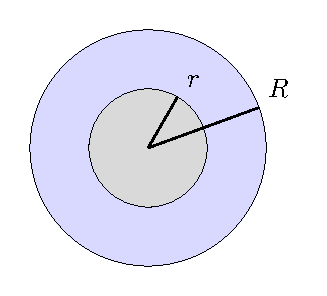
\includegraphics[width=0.4\textwidth]
{annulus_tikz_1}
\caption{\textbf{Paper roll viewed in cross-section} \\
The inner tube is shaded in gray, the layers of paper in blue (viewed in cross-section). 
\label{fig:annulus:01}}
\end{minipage}
\end{figure}

\newpage
\section*{Approach 1: Length from Area}
This is the approach shown by Professor Loh. It is ingenious because it calculates a circumference from an area and because the ``trick'' is visual.

In figure~\ref{fig:annulus:01}, the paper is rolled to a thickness of $(R-r)$cm. Between the inner tube (radius $r$) and the outer tube (radius $R$) are $300$ layers of paper. Professor Loh imagines that you unroll the paper and lay it flat. To picture this, imagine that instead of $300$ layers, we had a single layer (a very thick layer!). Figure~\ref{fig:annulus:02} shows what the unrolled layer would look like. The area of the annulus in the first picture is readily calculated as the difference between the area of the circle of radius $R$ and of the circle of radius $r$. The area of the rectangle in the second picture is the product of the length $L$ by the width $R-r$. The two are equal:
\begin{align*}
L(R-r) & = \pi(R^{2}-r^{2}) \\ 
\Rightarrow 
L & = \frac{\pi(R^{2}-r^{2})}{R-r}
\end{align*}

The reasoning is unchanged if there are $300$ layers. The length of the paper in this case is $300L$. The thinner the paper, the longer it must be. 

\begin{figure}[hpbt]
\begin{minipage}[b]{\textwidth}
\centering
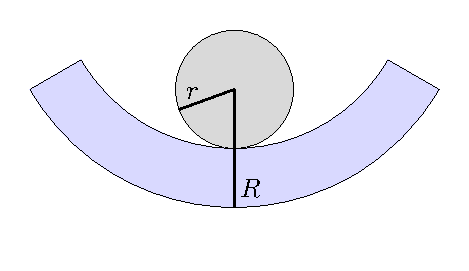
\includegraphics[width=0.4\textwidth]
{annulus_tikz_2}
\caption{\textbf{Unrolling the paper roll} \\
The inner tube is shaded in gray, the layers of paper in blue (viewed in cross-section). \\
{\footnotesize [the cut and lengths are approximate here]}
\label{fig:annulus:02}}
\end{minipage}
\end{figure}


\newpage
\section*{Approach 2: Length from Circumference}
This is perhaps the most natural approach for someone schooled in calculating circumferences of circles. The circumference of a circle of radius $r$ is $2\pi r$. The circumference of a circle of radius $R$ is $2\pi R$. Instinct suggests using the average of $r$ and $R$:
\begin{align*}
L = 2 \pi \left(\frac{r+R}{2}\right) = \pi (R + r)
\end{align*}
And for $300$ layers, that gives total length $300L$.

Is it appropriate to use the average radius? Any layer above it will have greater length, while any layer below it will have smaller length. But the differences cancel out! To see this, consider a layer of radius $m=(R+r)/2$, a layer of radius $m+\delta$ and a layer of radius $m-\delta$. See Figure~\ref{fig:annulus:03} The layer $m+\delta$ adds to the average length, while the layer $m-\delta$ subtracts from it. These are their circumferences:
\begin{align*}
& 2 \pi (m-\delta) \\
& 2 \pi (m+\delta) \\
\end{align*}
Adding these up, the $\delta$ cancels out. Thus, the outer layer adds to the average length exactly the amount that inner layer subtracts from it. Therefore the average radius gives the correct average length. 

\begin{figure}[hpbt]
\begin{minipage}[b]{\textwidth}
\centering
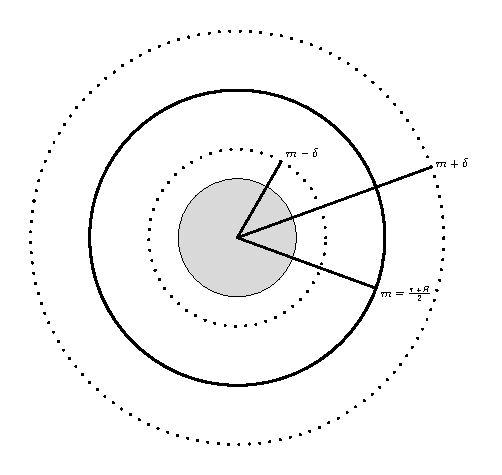
\includegraphics[width=0.4\textwidth]
{annulus_tikz_3b}
\caption{\textbf{Average layer.} \\
The inner tube is shaded in gray. The circumference of the average layer is the black continuous line. The dotted lines mark layers above and below the average, at a radial distance $\delta$.
\label{fig:annulus:03}}
\end{minipage}
\end{figure}

\newpage 
\section*{Reconciling Different Formulae}
How can we reconcile the two answers? We can check numerically. Or use this little ``trick'':
\begin{align*}
(R+r)(R-r) = R^{2}-r^{2}
\end{align*}
This is easy to verify from left to right. And now we can connect the two approaches:
\begin{align*}
L & = \frac{\pi(R^{2}-r^{2})}{R-r} \\
  & = \frac{\pi(R+r)(R-r)}{R-r} \\
  & = \pi (R+r)
\end{align*}

The advantage of Professor Loh's approach is that it is visual. Once you ``see'' the uncoiling process, it becomes clear how to connect the formula for the area of a circle with the formula for the area of a rectangle. The advantage of the second approach is that it does not involve squares. 

There are little difficulties with both approaches: On the one hand, if you uncoil a thick annulus you will see that the shape obtained is a trapezoid, not a rectangle (but for vanishingly thin layers, the difference does not matter). On the other hand, if you follow your instinct and calculate the circumference for the average radius, you will have to justify the simplification (as we did by considering what happens immediately above and below $m$). 
\end{document}